% !TeX spellcheck = cs_CZ
%{\tikzset{external/prefix={tikz/FYZI/}}
% \tikzset{external/figure name/.add={ch34_}{}}
%=========================== Kapitola: Relativistické jevy a záření ===============================
\chapter{Relativistické jevy a záření}\label{fyz:IchapXXXIV}
\minitoc
  \section{Pohybující se zdroje}\label{fyz:IchappXXXIVsecI}
  \section{\uv{Zdánlivý} pohyb}\label{fyz:IchappXXXIVsecII}
  \section{Synchrotronové záření}\label{fyz:IchappXXXIVsecIII}
  \section{Kosmické synchrotronové záření}\label{fyz:IchappXXXIVsecIV}
  \section{Brzdné záření}\label{fyz:IchappXXXIVsecV}
  \section{Dopplerův jev}\label{fyz:IchappXXXIVsecVI}
    V případě světla víme, že \(k_0 = \omega_0/c\), takže máme
    \begin{equation}\label{fyz:eq531}
      \omega = \omega_0\dfrac{1+\dfrac{v}{c}}{\sqrt{1-\dfrac{v^2}{c^2}}},
    \end{equation}
  \section{Vlnový čtyřvektor}\label{fyz:IchappXXXIVsecVII}
  \section{Aberace}\label{fyz:IchappXXXIVsecVIII}
  \section{Hybnost světla}\label{fyz:IchappXXXIVsecIX}
  \section{Příklady a cvičení}\label{fyz:IchappXXXIVsecX}

  \begin{figure}[ht!] %\ref{fyz:fig503}
    \centering
    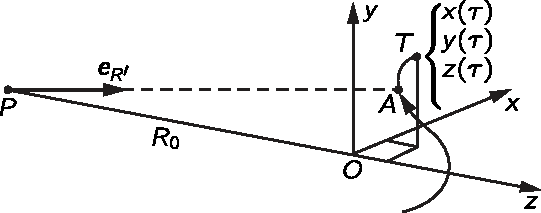
\includegraphics[width=0.9\linewidth]{fyz_fig503.pdf}
    \caption{
             (\cite[s.~697]{Feynman01})}
    \label{fyz:fig503}
  \end{figure}

  \begin{figure}[ht!] %\ref{fyz:fig504}
    \centering
    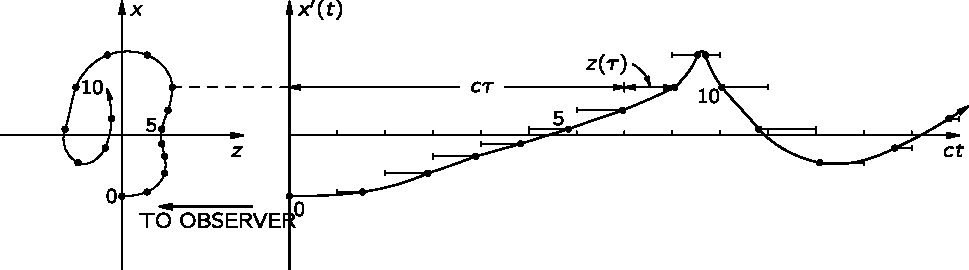
\includegraphics[width=1\linewidth]{fyz_fig504.pdf}
    \caption{
             (\cite[s.~697]{Feynman01})}
    \label{fyz:fig504}
  \end{figure}

  \begin{figure}[ht!] %\ref{fyz:fig505}
    \centering
    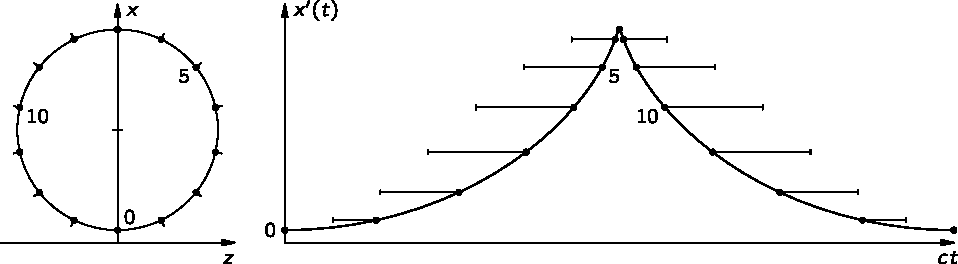
\includegraphics[width=1\linewidth]{fyz_fig505.pdf}
    \caption{
             (\cite[s.~697]{Feynman01})}
    \label{fyz:fig505}
  \end{figure}
  
  \begin{figure}[ht!] %\ref{fyz:fig506}
    \centering
    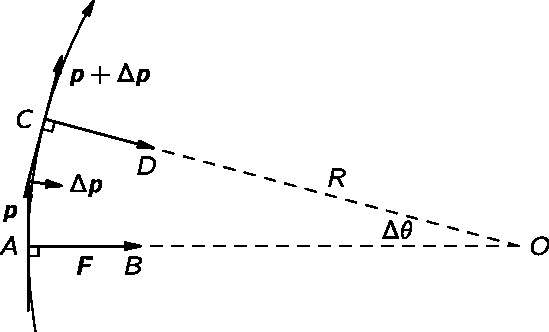
\includegraphics[width=0.9\linewidth]{fyz_fig506.pdf}
    \caption{
             (\cite[s.~697]{Feynman01})}
    \label{fyz:fig506}
  \end{figure}

  \begin{figure}[ht!] %\ref{fyz:fig507}
    \centering
    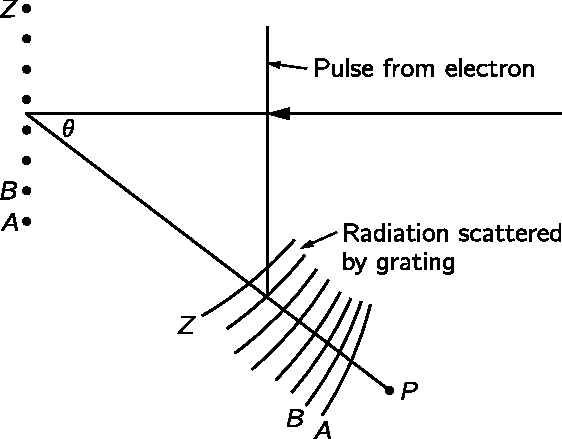
\includegraphics[width=0.9\linewidth]{fyz_fig507.pdf}
    \caption{
             (\cite[s.~697]{Feynman01})}
    \label{fyz:fig507}
  \end{figure}

  \begin{figure}[hb!] %\ref{fyz:fig508}
    \centering
    \begin{tabular}{c}
     \subfloat[ ]{\label{fyz:fig508a}
       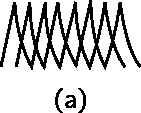
\includegraphics[width=0.6\linewidth]{fyz_fig508a.pdf}}  \\
     \subfloat[ ]{\label{fyz:fig508b}
       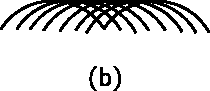
\includegraphics[width=0.6\linewidth]{fyz_fig508b.pdf}}  
    \end{tabular}
    \caption{
             (\cite[s.~601]{Feynman01}).}
    \label{fyz:fig508}
  \end{figure}

  \begin{figure}[ht!] %\ref{fyz:fig509}
    \centering
    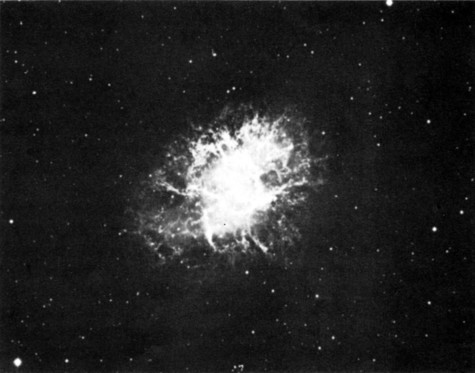
\includegraphics[width=0.6\linewidth]{fyz_fig509.jpg}
    \caption{
             (\cite[s.~697]{Feynman01})}
    \label{fyz:fig509}
  \end{figure}

  \begin{figure}[hb!] %\ref{fyz:fig510}
    \centering
    \begin{tabular}{c}
     \subfloat[ ]{\label{fyz:fig510a}
       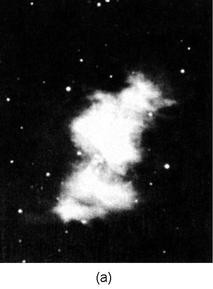
\includegraphics[width=0.7\linewidth]{fyz_fig510a.jpg}}  \\
     \subfloat[ ]{\label{fyz:fig510b}
       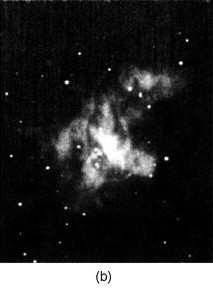
\includegraphics[width=0.7\linewidth]{fyz_fig510b.jpg}}  
    \end{tabular}
    \caption{
             (\cite[s.~601]{Feynman01}).}
    \label{fyz:fig510}
  \end{figure}

  \begin{figure}[hb!] %\ref{fyz:fig511}
    \centering
    \begin{tabular}{c}
     \subfloat[ ]{\label{fyz:fig511a}
       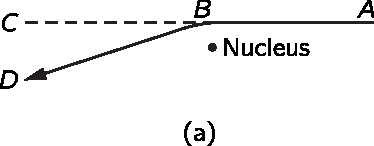
\includegraphics[width=0.7\linewidth]{fyz_fig511a.pdf}}  \\
     \subfloat[ ]{\label{fyz:fig511b}
       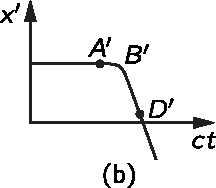
\includegraphics[width=0.5\linewidth]{fyz_fig511b.pdf}}  
    \end{tabular}
    \caption{
             (\cite[s.~601]{Feynman01}).}
    \label{fyz:fig511}
  \end{figure}

  \begin{figure}[hb!] %\ref{fyz:fig512}
    \centering
    \begin{tabular}{c}
     \subfloat[ ]{\label{fyz:fig512a}
       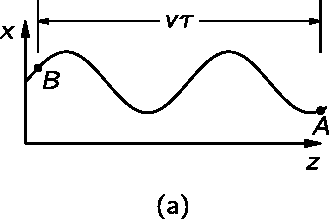
\includegraphics[width=0.7\linewidth]{fyz_fig512a.pdf}}  \\
     \subfloat[ ]{\label{fyz:fig512b}
       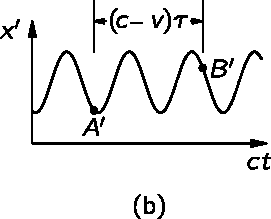
\includegraphics[width=0.7\linewidth]{fyz_fig512b.pdf}}  
    \end{tabular}
    \caption{
             (\cite[s.~601]{Feynman01}).}
    \label{fyz:fig512}
  \end{figure}

  \begin{figure}[ht!] %\ref{fyz:fig513}
    \centering
    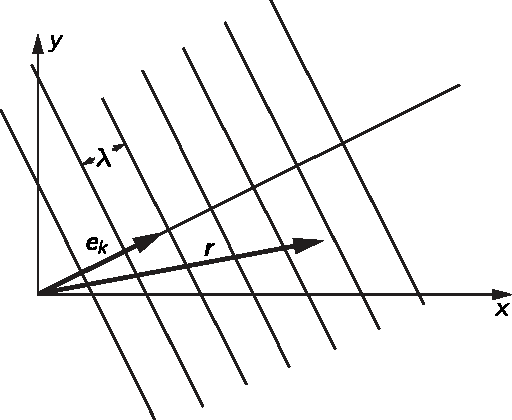
\includegraphics[width=0.8\linewidth]{fyz_fig513.pdf}
    \caption{
             (\cite[s.~697]{Feynman01})}
    \label{fyz:fig513}
  \end{figure}

  \begin{figure}[ht!] %\ref{fyz:fig514}
    \centering
    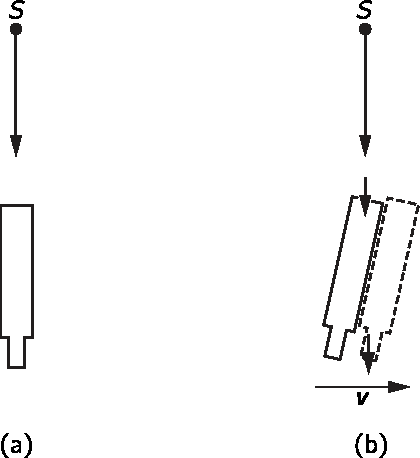
\includegraphics[width=0.7\linewidth]{fyz_fig514.pdf}
    \caption{
             (\cite[s.~697]{Feynman01})}
    \label{fyz:fig514}
  \end{figure}

  \begin{figure}[ht!] %\ref{fyz:fig515}
    \centering
    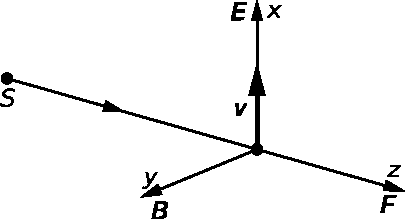
\includegraphics[width=0.6\linewidth]{fyz_fig515.pdf}
    \caption{
             (\cite[s.~697]{Feynman01})}
    \label{fyz:fig515}
  \end{figure}
  
%} %tikzset
%---------------------------------------------------------------------------------------------------
\printbibliography[title={Seznam literatury}, heading=subbibliography]
\addcontentsline{toc}{section}{Seznam literatury}